\documentclass{article}
\usepackage{graphicx}
\graphicspath{ {C:/Users/Finlay/Pictures/} }


\usepackage{Sweave}
\begin{document}

\title{My First Document}
\author{Finlay Campbell}

\maketitle

\begin{abstract}
	How are you doing, LaTeX?
\end{abstract}

\section{Introduction}
	This is the introduction of my first LaTeX document, I hope you enjoy it.
	
\begin{equation}
	\label{This is an equation}	
	\alpha = \sqrt{ \beta }
\end{equation}
	
\subsection{Finlay}
	This is first subsection of my first LaTeX document; I hope you enjoy this, too.

\section{Second Section}
	This is hopefully a big section, bigger than our Subsection 1.

\begin{figure}[!ht]
	\centering
	\includegraphics[width=3.0in]{Model.png}
	\caption{I don't think we have a figure yet}
\end{figure}

\section{Using Sweave to combine R and LaTeX}
Below we should see a plot rendered using R code.

\begin{figure}[tb]
	\centering
	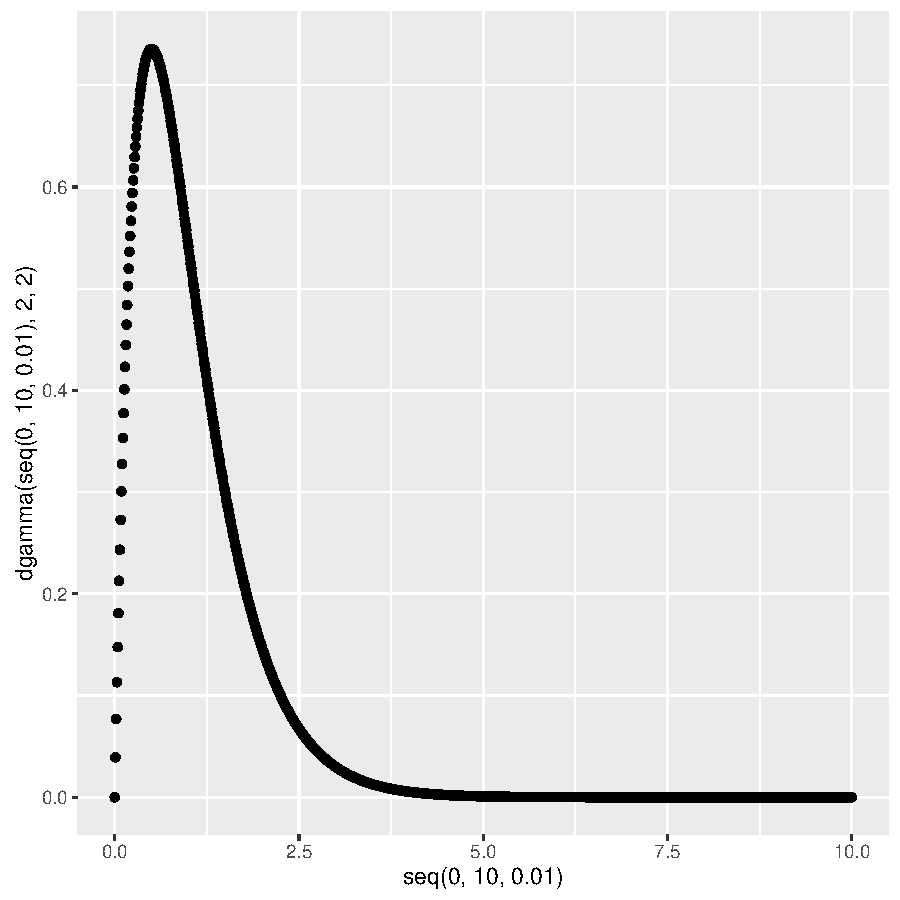
\includegraphics{sweave_test-ourplot}
	\caption{This is imported from R}
\end{figure}

Now we should be seeing normal text again. 


\section{Conclusion}
	This is the conclusion. 
	I hope you enjoyed this LaTeX document, come again. 

\end{document}
